\begin{equation}
\mathcal O\!\left(K(P_{\bm\theta}+MN+M^3)\right), \label{eq:onlinecomplex}
\end{equation}
plus one final forward evaluation of the same order. For a batch of $B$ samples,
an offline training iteration scales as
$\mathcal O(BK(P_{\bm\theta}+MN+M^3))$. Because the implemented outer update is
first-order, it does not store a full second-order graph through all $K$ inner
steps, reducing memory and derivative cost relative to full MAML. This is the
relevant complexity for \emph{prediction}: one compact network plus a fixed,
short RIS adaptation, rather than solving a fresh long alternating-optimization
problem from scratch for every channel.

%==============================================================================
\section{Numerical Results and Analysis}
Table~\ref{tab:sim} reports the parameters used by the fair NOMA-RIS simulator
and the final learning/evaluation scripts. The channel generator uses
$10{,}000$ realizations with a 90/10 train/validation split. The node geometry is
specified in the simulator by link distances rather than unique Cartesian
coordinates; reporting these distances therefore reproduces the propagation
model without inventing coordinates that are not present in the code.

\begin{table}[t]
\centering
\caption{System, channel, and learning parameters.}
\label{tab:sim}
\scriptsize
\begin{tabular}{@{}ll@{}}
\toprule
Parameter & Value \\ \midrule
BS antennas $M$ & 4 \\
RIS elements $N$ & 8 nominal; $\{8,16,32,64\}$ in RIS-size sweep \\
Power-sweep RIS size & $N=16$ \\
Monte-Carlo realizations & 10,000 (90\% train, 10\% validation) \\
BS--RIS distance $d_{BR}$ & 8 m \\
RIS--near distance $d_{RD_n}$ & 3 m \\
RIS--far distance $d_{RD_f}$ & 25 m \\
RIS--target / target--RIS & $d_{RT}=d_{TR}=6$ m \\
Direct BS--near / BS--far refs. & $d_{BD_n}=10$ m, $d_{BD_f}=25$ m \\
Reference path gain $PL_0$ & $10^{-3}$ ($-30$ dB) \\
Path-loss exponents & $2.2,2.8,2.8,2.3,2.3,3.8,3.8$ \\
Nakagami-$m$ parameters & $m_{BR}=2$, $m_{RD_n}=m_{RD_f}=1$; \\
 & $m_{RT}=m_{TR}=3$, $m_{BD_n}=m_{BD_f}=1$ \\
Target gain $\beta_T$ & 40 dB \\
RIS amplitude $\beta_i$ / efficiency & 1 / 1 (ideal passive RIS) \\
Bandwidth / temperature / NF & 1 MHz / 290 K / 6 dB \\
Generator power $P_{\rm tot}$ & 40 dBm; trainer permits power override \\
RIS-size figure operating power & 15 dBm \\
Power sweep & $5,10,15,20,25$ dBm \\
Initial NOMA split $(a_n,a_f,a_T)$ & $(0.20,0.55,0.25)$ \\
Communication beam weights & far/near $=0.7/0.3$ \\
Sensing leakage penalty $\lambda_{\rm null}$ & 0.5 \\
Objective weights $(\omega_c,\omega_s)$ & $(0.7,0.3)$ \\
NOMA cluster/sensing QoS & $R_{\rm th,c}=21.7$, $R_{\rm th,s}=2.9$ bit/s/Hz \\
Individual training floors & $R_{\rm th,n}=R_{\rm th,f}=1$ bit/s/Hz \\
Penalty weights $(\lambda_c,\lambda_s,\lambda_n,\lambda_f)$ & $(2,50,15,20)$ \\
Power network & 9--256--256--256--3, softmax output \\
NOMA-RIS result checkpoints & batch 64, lr $10^{-4}$, 40 epochs, $K=10$ \\
OMA-RIS result checkpoints & batch 64, lr $10^{-4}$, 40 epochs, $K=5$ \\
No-RIS result checkpoints & batch 128, lr $5\times10^{-4}$, 60 epochs \\
Inner phase optimizer & Adam, learning rate 0.1 \\
\bottomrule
\end{tabular}
\end{table}

The aggregate NOMA threshold in Table~\ref{tab:sim} comes from the fair NOMA
dataset, where it was chosen to keep the cluster QoS active; the individual
near/far floors are the defaults used by the training scripts. The OMA fair
dataset uses its own calibrated aggregate/sensing thresholds
($R_{\rm th,c}=12$ and $R_{\rm th,s}=2$ bit/s/Hz). The service-rate outage
thresholds stored by the MATLAB generators are diagnostic quantities and are
not the same as the optimization penalties in~\eqref{eq:sampleloss}.

The implementation records per-iteration loss and weighted rate for convergence
monitoring, while model selection uses a held-out validation score. The present
analysis therefore relies on the fixed-step inner optimizer, validation-based
checkpointing, and the convergence limitations discussed in
Section~III-E rather than asserting a closed-form global guarantee.

Fig.~\ref{fig:ablation} summarizes the NOMA ablation. The final CSV reports a
weighted sum-rate increase from 5.34 bit/s/Hz for random phase/random allocation
to 6.81 bit/s/Hz for joint optimization. The legacy reported joint QoS metric
(cluster communication plus sensing) drops from 29.38\% to 0.06\%. The
individual near/far penalties are included during training, but the legacy
$q_{\rm any}$ field used to draw this figure does not count individual-user
violations; this distinction is stated explicitly to avoid interpreting the
0.06\% number as a per-user outage probability.

\begin{figure}[t]
  \centering
  \subfloat[Weighted sum-rate.]{%
  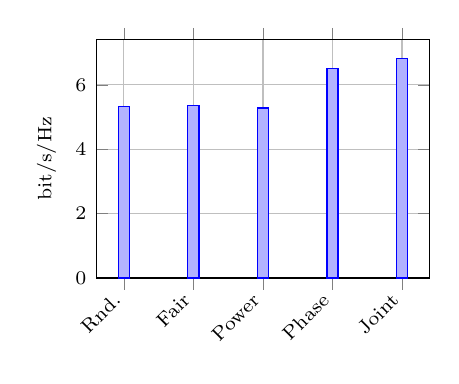
\begin{tikzpicture}
  \begin{axis}[
    width=0.48\columnwidth,height=0.38\columnwidth,
    ybar,bar width=4pt,ymin=0,ymax=7.4,
    ylabel={bit/s/Hz},
    symbolic x coords={R,F,P,Q,J},xtick=data,
    xticklabels={Rnd.,Fair,Power,Phase,Joint},
    x tick label style={rotate=45,anchor=east,font=\scriptsize},
    tick label style={font=\scriptsize},label style={font=\scriptsize},
    grid=major]
  \addplot coordinates {(R,5.3397) (F,5.3484) (P,5.2819) (Q,6.5045) (J,6.8073)};
  \end{axis}
  \end{tikzpicture}}\hfill
  \subfloat[QoS violation.]{%
  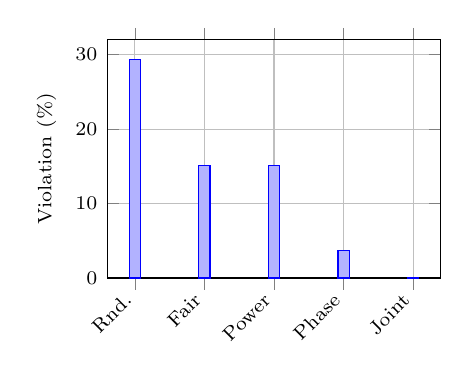
\begin{tikzpicture}
  \begin{axis}[
    width=0.48\columnwidth,height=0.38\columnwidth,
    ybar,bar width=4pt,ymin=0,ymax=32,
    ylabel={Violation (\%)},
    symbolic x coords={R,F,P,Q,J},xtick=data,
    xticklabels={Rnd.,Fair,Power,Phase,Joint},
    x tick label style={rotate=45,anchor=east,font=\scriptsize},
    tick label style={font=\scriptsize},label style={font=\scriptsize},
    grid=major]
  \addplot coordinates {(R,29.38) (F,15.12) (P,15.10) (Q,3.70) (J,0.06)};
  \end{axis}
  \end{tikzpicture}}
  \caption{Ablation of power and phase optimization. The QoS panel uses the
  legacy aggregate-communication/sensing violation metric. ``Power'' denotes
  learned power with random phase; ``Phase'' denotes optimized phase with
  random power.}
  \label{fig:ablation}
\end{figure}

Fig.~\ref{fig:rateN} varies $N\in\{8,16,32,64\}$. The NOMA-RIS weighted
sum-rate rises from 6.85 to 11.45 bit/s/Hz and the OMA-RIS rate rises from 4.09
to 7.27 bit/s/Hz. The no-RIS curves are independent of $N$ and are therefore
shown as horizontal dashed reference lines, directly addressing the desired
``no RIS'' presentation. At the 15-dBm reference point the corresponding
no-RIS values are 6.58 bit/s/Hz for NOMA and 3.01 bit/s/Hz for OMA.

\begin{figure}[t]
  \centering
  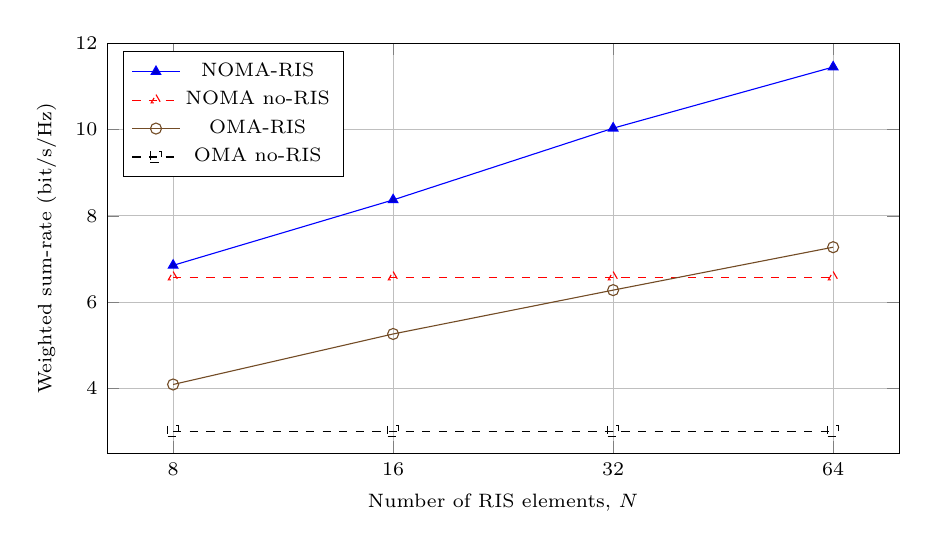
\begin{tikzpicture}
  \begin{axis}[
    width=0.96\columnwidth,height=0.56\columnwidth,
    xlabel={Number of RIS elements, $N$},
    ylabel={Weighted sum-rate (bit/s/Hz)},
    xmode=log,log basis x=2,xtick={8,16,32,64},
    xticklabels={8,16,32,64},
    ymin=2.5,ymax=12,
    legend style={font=\scriptsize,at={(0.02,0.98)},anchor=north west},
    tick label style={font=\scriptsize},label style={font=\scriptsize},
    grid=major]
  \addplot+[mark=triangle*] coordinates {(8,6.8521) (16,8.3680) (32,10.0297) (64,11.4463)};
  \addlegendentry{NOMA-RIS}
  \addplot+[dashed,mark=triangle] coordinates {(8,6.5805) (16,6.5805) (32,6.5805) (64,6.5805)};
  \addlegendentry{NOMA no-RIS}
  \addplot+[mark=o] coordinates {(8,4.0929) (16,5.2630) (32,6.2786) (64,7.2729)};
  \addlegendentry{OMA-RIS}
  \addplot+[dashed,mark=square] coordinates {(8,3.0063) (16,3.0063) (32,3.0063) (64,3.0063)};
  \addlegendentry{OMA no-RIS}
  \end{axis}
  \end{tikzpicture}
  \caption{Weighted sum-rate versus RIS size at the 15-dBm reference power.
  Solid curves use the RIS; horizontal dashed curves are the no-RIS baselines.}
  \label{fig:rateN}
\end{figure}

Fig.~\ref{fig:rateP} sweeps the transmit power from 5 to 25 dBm for the
$N=16$ RIS configuration. At 15 dBm, NOMA-RIS achieves 8.37 bit/s/Hz versus
6.58 bit/s/Hz without the RIS, a gain of about 27\%. The corresponding OMA
values are 5.26 and 3.01 bit/s/Hz. The right panel also shows that the reported
aggregate/sensing QoS violation falls rapidly with power for the RIS-assisted
schemes. In both panels, no-RIS curves use dashed lines.

\begin{figure}[t]
  \centering
  \subfloat[Weighted sum-rate.]{%
  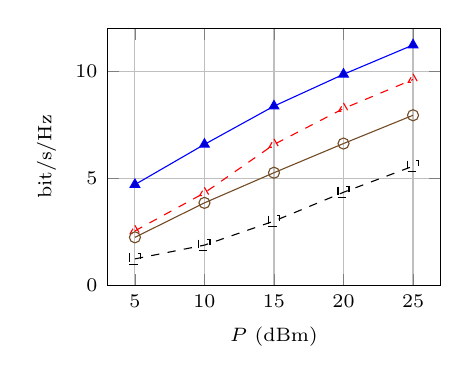
\begin{tikzpicture}
  \begin{axis}[
    width=0.48\columnwidth,height=0.40\columnwidth,
    xlabel={$P$ (dBm)},ylabel={bit/s/Hz},xtick={5,10,15,20,25},
    ymin=0,ymax=12,
    tick label style={font=\scriptsize},label style={font=\scriptsize},grid=major]
  \addplot+[mark=triangle*] coordinates {(5,4.7088) (10,6.5836) (15,8.3680) (20,9.8509) (25,11.2174)};
  \addplot+[dashed,mark=triangle] coordinates {(5,2.5493) (10,4.3220) (15,6.5805) (20,8.2545) (25,9.6096)};
  \addplot+[mark=o] coordinates {(5,2.2510) (10,3.8564) (15,5.2630) (20,6.6227) (25,7.9415)};
  \addplot+[dashed,mark=square] coordinates {(5,1.2449) (10,1.8866) (15,3.0063) (20,4.3509) (25,5.5677)};
  \end{axis}
  \end{tikzpicture}}\hfill
  \subfloat[QoS violation.]{%
  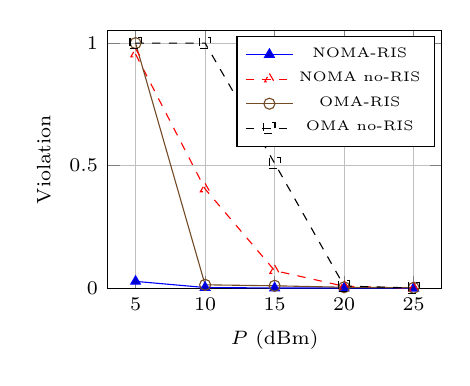
\begin{tikzpicture}
  \begin{axis}[
    width=0.48\columnwidth,height=0.40\columnwidth,
    xlabel={$P$ (dBm)},ylabel={Violation},xtick={5,10,15,20,25},
    ymin=0,ymax=1.05,
    legend style={font=\tiny,at={(0.98,0.98)},anchor=north east},
    tick label style={font=\scriptsize},label style={font=\scriptsize},grid=major]
  \addplot+[mark=triangle*] coordinates {(5,0.028) (10,0.003) (15,0.001) (20,0.001) (25,0)};
  \addlegendentry{NOMA-RIS}
  \addplot+[dashed,mark=triangle] coordinates {(5,0.955) (10,0.405) (15,0.072) (20,0.008) (25,0)};
  \addlegendentry{NOMA no-RIS}
  \addplot+[mark=o] coordinates {(5,1.000) (10,0.014) (15,0.010) (20,0.004) (25,0.002)};
  \addlegendentry{OMA-RIS}
  \addplot+[dashed,mark=square] coordinates {(5,1.000) (10,1.000) (15,0.510) (20,0.009) (25,0.001)};
  \addlegendentry{OMA no-RIS}
  \end{axis}
  \end{tikzpicture}}
  \caption{(a) Weighted sum-rate and (b) legacy aggregate/sensing QoS-violation
  fraction versus transmit power for NOMA/OMA with and without the RIS. Dashed
  curves denote no-RIS baselines.}
  \label{fig:rateP}
\end{figure}

%==============================================================================
\section{Conclusion}
A MISO RIS-assisted NOMA-ISAC downlink was investigated with joint power and
phase design. The revised formulation combines an aggregate NOMA-cluster QoS
constraint with individual near/far-user floors and a separate sensing floor,
which preserves cluster efficiency while preventing a strong user from masking
a weak one. The implemented solver uses a compact softmax power network and
per-channel RIS-phase adaptation, followed by a first-order meta-update. The
paper now reports the actual channel distances, fading/path-loss parameters,
power/RIS settings, convergence limitations, and online prediction complexity.
The regenerated RIS-size and power-sweep figures include explicit dashed no-RIS
baselines and are provided in both vector EPS and raster JPG forms.

%==============================================================================
\begin{thebibliography}{1}
\bibitem{liu2022isac}
F.~Liu \emph{et al.}, ``Integrated sensing and communications: Toward
dual-functional wireless networks for 6G and beyond,''
\emph{IEEE J. Sel. Areas Commun.}, vol.~40, no.~6, pp.~1728--1767, Jun.~2022.

\bibitem{deng2025mmwave}
K.~Deng, X.~Wang, H.~Xu, Q.~Song, R.~Zhang, and Y.~Qian, ``Balancing
communication and sensing hybrid beamforming with rank-1 optimization for
mmWave ISAC systems,'' \emph{IEEE Wireless Commun. Lett.}, vol.~14, no.~9,
pp.~2738--2742, Sep.~2025.

\bibitem{wu2020ris}
Q.~Wu and R.~Zhang, ``Towards smart and reconfigurable environment: Intelligent
reflecting surface aided wireless network,'' \emph{IEEE Commun. Mag.}, vol.~58,
no.~1, pp.~106--112, Jan.~2020.

\bibitem{wang2025hybrid}
L.~Wang, L.~F. Abanto-Leon, and A.~Asadi, ``Joint hybrid beamforming and RIS
phase shift design for RIS-enabled mmWave ISAC system,'' \emph{IEEE Trans. Veh.
Technol.}, vol.~74, no.~6, pp.~9149--9164, Jun.~2025.

\bibitem{lyu2024crb}
W.~Lyu \emph{et al.}, ``CRB minimization for RIS-aided mmWave integrated sensing
and communications,'' \emph{IEEE Internet Things J.}, vol.~11, no.~10,
pp.~18381--18393, May~2024.

\bibitem{ke2025rsma}
H.~Ke, J.~Xu, W.~Xu, C.~Ding, and D.~W.~K. Ng, ``Rate splitting and beamforming
design for RIS-assisted RSMA-enhanced ISAC networks,'' \emph{IEEE Wireless
Commun. Lett.}, vol.~14, no.~6, pp.~1738--1742, Jun.~2025.

\bibitem{zou2023ml}
Y.~Zou, Y.~Liu, X.~Mu, X.~Zhang, Y.~Liu, and C.~Yuen, ``Machine learning in
RIS-assisted NOMA IoT networks,'' \emph{IEEE Internet Things J.}, vol.~10,
no.~22, pp.~19427--19440, Nov.~2023.

\bibitem{wei2026ris}
T.~Wei \emph{et al.}, ``Machine learning-driven joint RIS partitioning,
beamforming, and phase shifts design for mmWave ISAC systems,'' \emph{IEEE
Wireless Commun. Lett.}, vol.~15, 2026.

\bibitem{maml}
C.~Finn, P.~Abbeel, and S.~Levine, ``Model-agnostic meta-learning for fast
adaptation of deep networks,'' in \emph{Proc. ICML}, 2017, pp.~1126--1135.

\bibitem{fallah2020maml}
A.~Fallah, A.~Mokhtari, and A.~Ozdaglar, ``On the convergence theory of
gradient-based model-agnostic meta-learning algorithms,'' in \emph{Proc.
AISTATS}, 2020, pp.~1082--1092.

\bibitem{ji2022maml}
K.~Ji, J.~Yang, and Y.~Liang, ``Theoretical convergence of multi-step
model-agnostic meta-learning,'' \emph{J. Mach. Learn. Res.}, vol.~23, pp.~1--41,
2022.

\bibitem{sun2024noma}
Y.~Sun \emph{et al.}, ``On the study of NOMA-assisted integrated sensing and
communication networks,'' \emph{IEEE Trans. Commun.}, vol.~72, no.~11,
pp.~7278--7293, Nov.~2024.
\end{thebibliography}

\end{document}
